%!TEX root = ../thesis.tex

\section{Cassandra}
\label{sec:theory:cassandra}
% TODO referencje do Cassandry, krotki wstep o Cassandrze
% TODO wspomnieć o LWT.
Cassandra \cite{CassandraApacheDocs} \cite{CassandraDataStaxDocs} \cite{lakshman2010cassandra} is a high performance, scalable, fault tolerant (i.e. no single point of failure), distributed post-relational database solution, which combines benefits of Google Bigtable \cite{chang2008bigtable} and Amazon Dynamo \cite{decandia2007dynamo}.
% to handle the types of database management needs that traditional RDBMS vendors cannot support. 

%Cassandra offers linear scale performance, which means that, for example if four nodes can handle hundred thousand 
%requests per second, then adding another four nodes results in the cluster, which can handle twice as much requests per second. Cassandra provides continous availability, due to redundancy of both data and node functions, which eliminate SPOF and provide constant uptime. 

\subsection{Key features}
Its key features are:
\begin{enumerate*}
\item masterless architecture,
\item linear scale performance \ref{sec:theory:cassandra:linear},
\item continuous availability,
\item flexible data model \ref{sec:theory:cassandra:datamodel},
\item multi data center support,
\item all nodes accept reads and writes,
\item Cassandra Query Language \ref{sec:theory:cassandra:cql}.
\end{enumerate*}

\subsection{Architecture}
Cassandra has a masterless \emph{ring} architecture \ref{fig:archCluster}, in which all nodes are equally significant, and there is no master node, therefore there is no single point of failure (SPOF). Cassandra uses replication, which is keeping copies of the data on multiple nodes, to also avoid SPOF during reads and writes. Cassandra provides continous availability, due to redundancy of both data and node functions, which eliminate SPOF and provide constant uptime.
Cassandra supports \emph{gossip} protocol, which is a scalable, distributed protocol used for inter-node communication.

\begin{figure}[h]
	\centering
	%\subfloat[The cluster on the ring]
	%{
	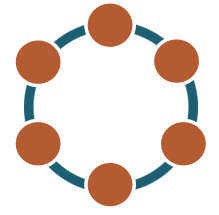
\includegraphics[height=60mm]{images/cassandra-ring.png}\hspace{10mm}
	%}	
	\caption{A cluster on the ring}
	\label{fig:archCluster}
\end{figure}

\subsection{Replication}
Cassandra supports configurable replication via \emph{replication factor N}, which is the total number of nodes on which the data is stored, defined per \emph{keyspace} \ref{sec:theory:cassandra:datamodel}. A replication factor of $3$ means that three copies of the data exist across the cluster on $3$ different nodes.

Figure \ref{fig:replicationRing} shows a replication of the token $91$ in the cluster with $4$ nodes and the token ring with tokens ranging from $0$ to $99$. 
Each node is the \emph{primary replica} for the token range placed counter clock-wise to it, thus node $1$ is the primary replica for range $75-0$, node $2$ for $1-25$, node $3$ for $26-50$, and node $4$ for $51-75$. 
Token value $91$ belongs to the node $1$, and since $N=3$, then the value is replicated on $2$ more nodes, which are on counter wise positions, thus on node $2$ and node $3$, which are \emph{secondary replicas} of the token. 

% źródło https://pandaforme.gitbooks.io/introduction-to-cassandra/content/understand_replication.html
% prawdziwe źródło to prawdopodobnie kurs z DataStax, ale nie mogę tego znaleźć.
\begin{figure}[h]
	\centering
	%\subfloat[The cluster on the ring]
	%{
	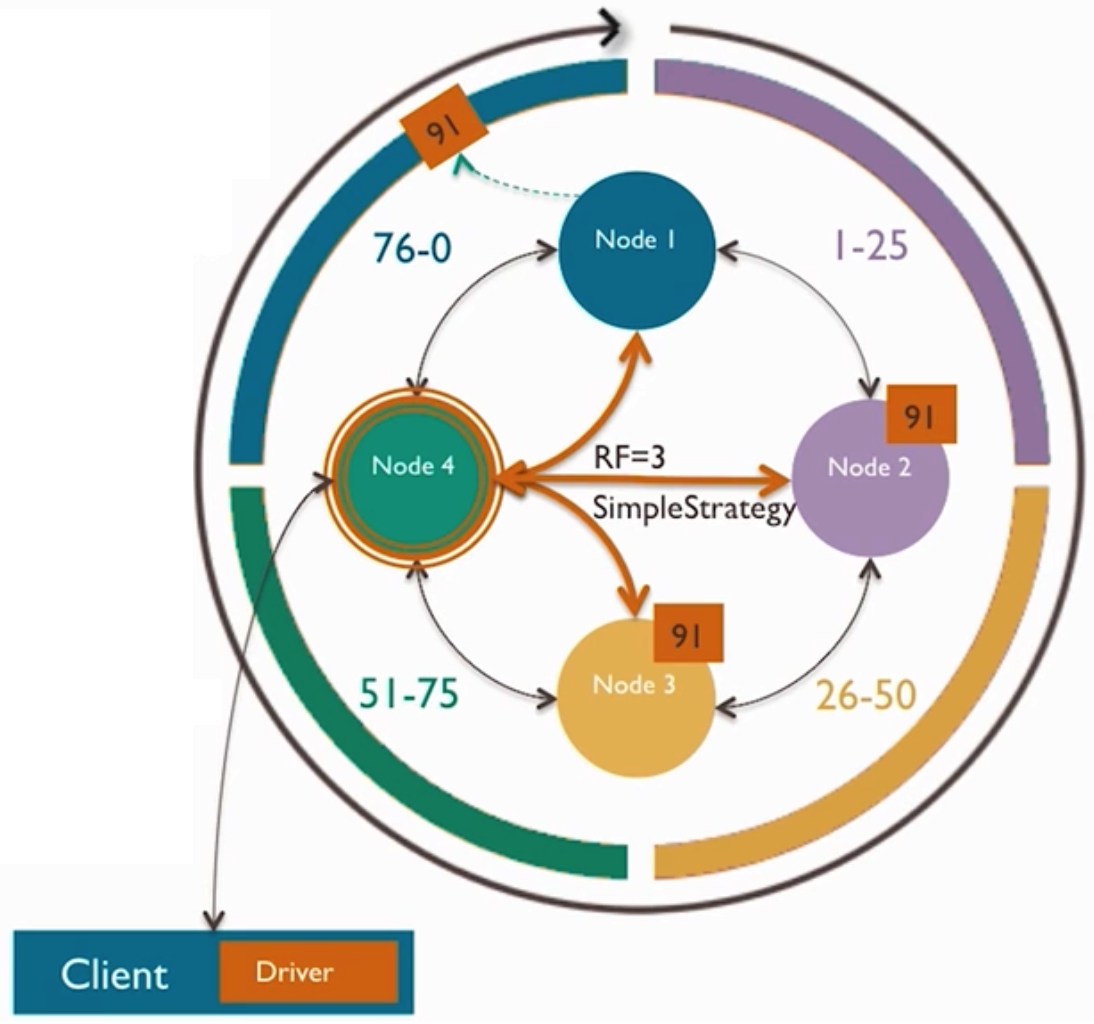
\includegraphics[height=100mm]{images/cassandra-replication-ring.png}\hspace{10mm}
	%}
	%\label{fig:replicationRing}
	\caption{Replication of the token 91}
	\label{fig:replicationRing}
\end{figure}

%\subsubsection{Read path}
%TODO Read path
%\subsubsection{Write path}
%TODO Write path

%Architecture
% Token ring
% rysunek z klastrem



\subsection{Data model}
\label{sec:theory:cassandra:datamodel}
Cassandra's data model is a wide-row store, which consists of tables, which reside in keyspaces\footnote{comparable to schemas in RDBMS} with rows, identified by primary keys, with up to 2 billion columns. Although data model concepts are similar to relational ones, data modeling techniques depart from the relational modeling, since models are supposed to be highly denormalized, which provide ability to perform fast queries by reading a single partition, which is the unit of the data replication in Cassandra, in order to fetch all the data the query needs without further communication with other nodes and performing joins\footnote{which do not exist in Cassandra}.

%\begin{description}
%\item[keyspace] 
%\item[table]
%\item[column]
%\item[row]
%\item[primary key]
%\end{description}

\subsection{Linear scale performance}
\label{sec:theory:cassandra:linear}
Cassandra offers linear scale performance, which means that if two nodes can handle hundred thousand requests per second, then adding another two nodes results in the cluster, which can handle twice as much requests per second. Figure \ref{fig:archLinearScale} depicts the example.

The key principles behind linear scaling are:  data partitioning and token ranges. 
Partitioning is the assignment of the token values, which are \emph{long} values, to the keys, and more concretely to the partitioning keys of a primary key. Cassandra provides different \emph{Partitioners}, which implement different algorithms to perform such token assignment. \emph{Murmur3Partitioner} uses \emph{Murmur3} hash algorithm that provides a good distribution over the hash space, and is fast due to the fact that it does not support cryptographic properties, which are not required by Cassandra.

Each node is responsible for a token range, which is a part of the token ring. Responsibility means that a node stores the data for which the token value falls into its token range. When a new node is added, it automatically receives a token range and then the data is moved between the nodes in order to adjust to the new division of the token ring.

Correct data modeling is also an important aspect of the linear scalability, since partitioning keys of tables have to be designed in a way that provides high cardinality of the keys. Otherwise part of the cluster starts to collect more data than its storage capabilities, and it will fail. 


\begin{figure}[H]
  \centering  
  % TODO źródło?
  % Źródło http://docs.datastax.com/en/cassandra/2.1/cassandra/images/intro_cassandra.png
  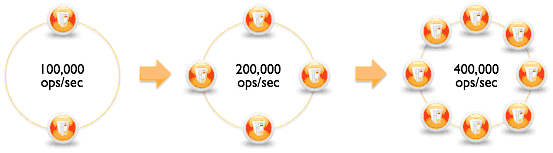
\includegraphics[width=\textwidth]{images/cassandra-linear-scalability.png}\hspace{10mm}  
  \caption{The linear scalability from 100k to 200k requests per second}
  \label{fig:archLinearScale}
\end{figure}


%Linear scale performance is provided by even assignment of token ranges of the token ring to the nodes in the cluster combined with data \emph{partitioning} -- which is assigning a token values to the keys -- that evenly distributes the data around the cluster. When a new node is added to the cluster, it automatically 


\subsection{Cassandra Query Language}
\label{sec:theory:cassandra:cql}
Cassandra Query Language (CQL) is the query language, similar in syntax to SQL, but provides only limited functionality compared to SQL, as there are no joins, inner queries, nor aggregations. CQL provides select, insert, update and delete statements. Select statement's \emph{where} clause supports equality condition on the partition key columns and restrictions such as: IN, =, >, >=, <= and < on the clustering columns. Columns, which are not part of the primary key cannot be restricted in the \emph{where} clause. Listing \ref{lst:cqlSelect} shows two examples of select statements, first with equality restriction on the partition key column \emph{user_id}, second with equality restrictions on the partition key columns: \emph{cluster}, \emph{date}, \emph{datacenter}, and range restrictions on the clustering key columns: \emph{hour} and \emph{minute}.
%Cassandra uses binary protocol named Cassandra Query Language (CQL). In order to do anything with database, we need to use a driver that speaks binary protocol. 

\begin{lstlisting}[style=outcode,label={lst:cqlSelect},caption={Examples of CQL select statements}]
SELECT user_name, user_email 
FROM app.users 
WHERE user_id = 10123;
    
SELECT * FROM app.requests
 WHERE cluster = 'cluster1'
 AND date = '2015/06/05'
 AND datacenter = 'EU_NORTH'
 AND (hour, minute) >= (12, 0) AND (hour, minute) <= (15, 30);
\end{lstlisting}

 
\subsection{Use cases}
Cassandra is a general purpose non-relational database, however there are areas in which Cassandra excels over other databases:
\begin{enumerate*}
\item internet of things applications - Cassandra is able to consume large quantity of incoming data\footnote{depends on cluster size} from devices, sensors and similar internet connected devices,
%\item E-commerce - durable shopping cart protection combined with fast product catalog browsing
%\item Messaging - Cassandra serves as the database for mobile phone applications
\item data analytics - Cassandra provides storage with fast access to the data for analysis. Apache Spark, which is an engine to perform large-scale data processing \cite{ApacheSpark} supports Cassandra, as one of its data sources, therefore Cassandra provides data storage for analytics and also stores results of the analysis done in Spark,
\item storage of time series data - Cassandra's fast writes, wide-rows and ability to read only particular data ranges are well suited for time series based applications, because such data fits natively into the data model.
\end{enumerate*} 

\subsection{Transactions}
Cassandra does not provide ACID compliant transactions, but it offers Light Weight Transactions, which offer a degree of transactionality limited to the scope of single partition, therefore to the single primary key\footnote{concretely to the partitioning part of the key in terms of the complex key}. Section \ref{sec:theory:transactions:lwt} provides more on this subject in comparison to other distributed transactions. 

\subsubsection{Compared to RDBMS}
\begin{figure}[hbt]
  %\centering
  \setlength{\unitlength}{1.3cm}  
  \subfloat{
    \renewcommand{\tabcolsep}{0.1cm}
    \resizebox{\textwidth}{!}{\begin{tabular}{c|c}
      \toprule
      RDBMS & Cassandra  \\ \midrule
      manages structured data      &  manages any type of data    \\
      ACID transactions 		   &  simple transactions supported by LWT \\
      SQL & CQL \\
      scales vertically & scales horizontally \\
      master-slave architecture & masterless, share nothing architecture \\
      denormalization is the bad practice & denormalization is the best practice \\
      single points of failure with failover & no single points of failure \\  \bottomrule      
    \end{tabular}}
  }
  \caption{RDBMS compared to Cassandra}
  \label{fig:cassandraToRdbms}
\end{figure}

\subsection{Eventual consistency}\label{sec:theory:eventualConsistency}
In terms of CAP \cite{brewer2000towards} \cite{Brewer:2012ba} Cassandra is the \emph{AP} database with eventual consistency, which means that over time the data becomes consistent on all nodes, but there are no guarantees about the time it takes. Cassandra uses techniques such as: \begin{enumerate*} 
\item \emph{hinted handoff} - stores a message for the currently unavailable replica about the modification and sends it to the replica when it comes back up \cite{CassandraHintedHandoff},  
\item \emph{read repairs} - detects inconsistency in the data during read and repairs it by sending a message with the data \cite{CassandraReadRepair},  \end{enumerate*} to pro-actively reduce incosistency in the data during normal operations.